% command for a new time slot
\newcommand{\talktime}{9:99}
\newcommand{\newtimeslot}[1]{\newpage\renewcommand{\talktime}{#1}}

% new time slot but without a pagebreak
\newcommand{\newsmalltimeslot}[1]{\renewcommand{\talktime}{#1}}

% initialise \conferenceDay 
\newcommand{\conferenceDay}{Noday}


% define default page style (cutting marks with page number)
\DeclareNewLayer[background, oddorevenpage, width=125mm,%
height=169mm, contents={%
  
\includegraphics{wallpaper/crop-marks.pdf}%
}]{cropmarksevery}
\newpairofpagestyles[scrheadings]{cropmarksstyle}{}
\AddLayersAtBeginOfPageStyle{cropmarksstyle}{cropmarksevery}

% page style for title pages
\DeclareNewLayer[background, oddorevenpage, width=125mm,%
height=169mm, contents={%
  
\includegraphics{wallpaper/front-cover-with-crop-marks.pdf}%
}]{titlelayer}
\newpairofpagestyles[]{titlestyle}{}
\AddLayersAtBeginOfPageStyle{titlestyle}{titlelayer}

% define alias commands for all three days
\def\saturday{Saturday}
\def\sunday{Sunday}
\def\monday{Monday}

% define Saturday page style
\DeclareNewLayer[background, oddpage,  width=125mm,%
height=169mm, contents={%
  
\includegraphics{wallpaper/saturday-odd.pdf}%
}]{saturdayodd}
\DeclareNewLayer[background, evenpage,  width=125mm,%
height=169mm, contents={%
  
\includegraphics{wallpaper/saturday-even.pdf}%
}]{saturdayeven}
\DeclareNewLayer[background, oddpage,  width=125mm,%
height=169mm, contents={%
  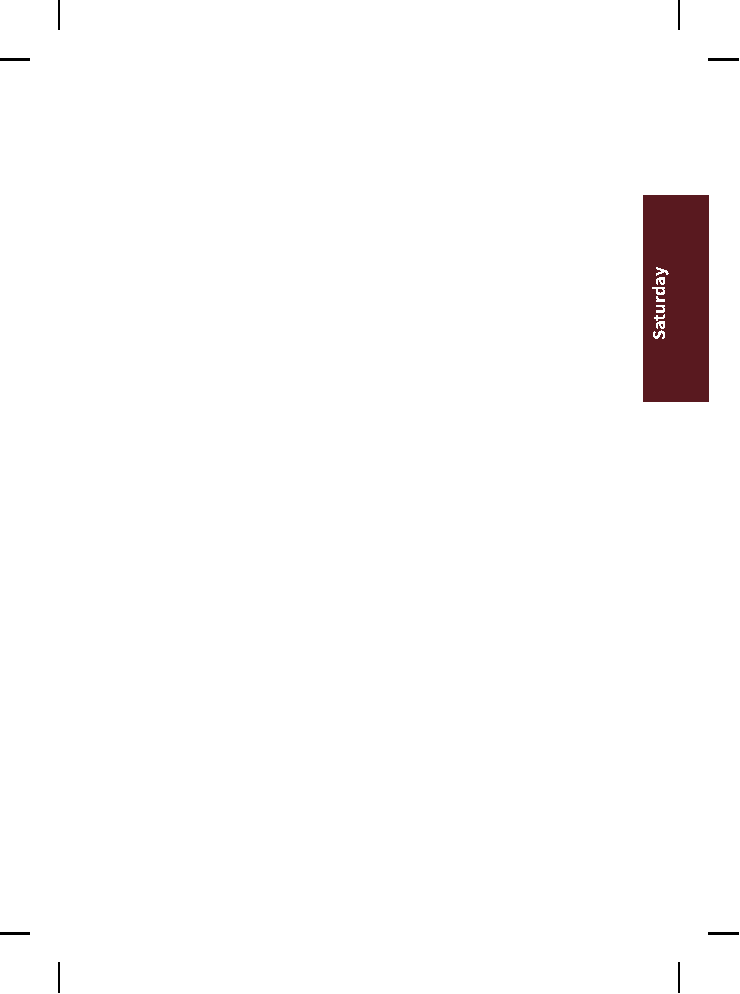
\includegraphics{wallpaper/saturday-odd-rotated.pdf}%
}]{saturdayoddrotated}
\newpairofpagestyles[scrheadings]{saturday-table}{}
\AddLayersAtBeginOfPageStyle{saturday-table}{saturdayeven}
\AddLayersAtBeginOfPageStyle{saturday-table}{saturdayoddrotated}
\newpairofpagestyles[scrheadings]{saturday}{}
\AddLayersAtBeginOfPageStyle{saturday}{saturdayeven}
\AddLayersAtBeginOfPageStyle{saturday}{saturdayodd}

% define Sunday page style
\DeclareNewLayer[background, oddpage,  width=125mm,%
height=169mm, contents={%
  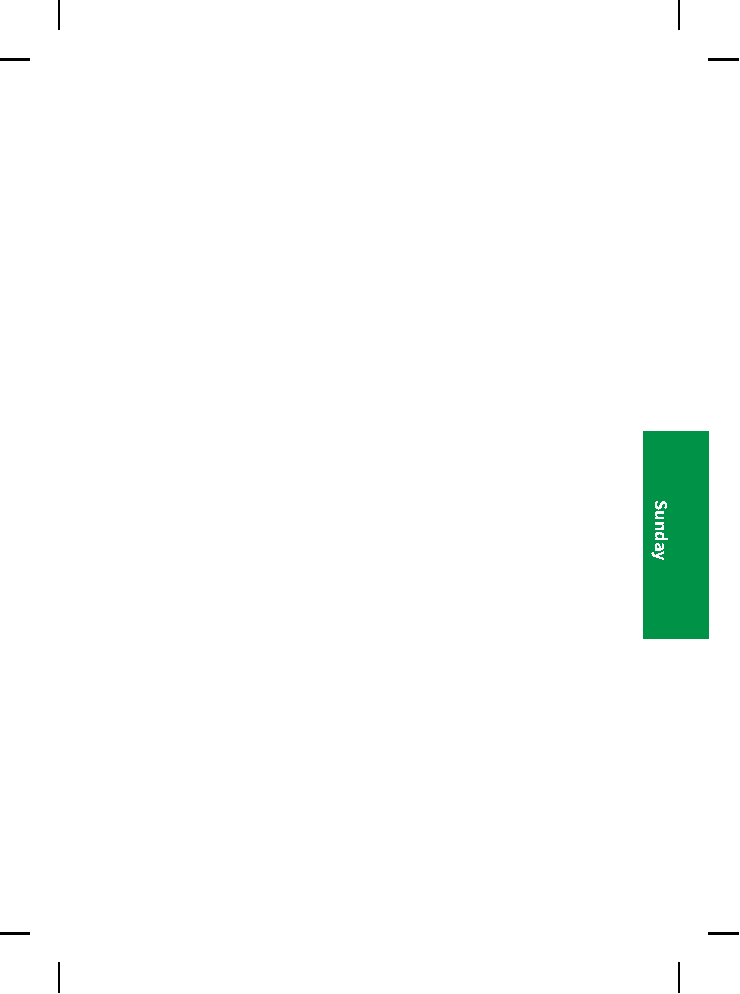
\includegraphics{wallpaper/sunday-odd.pdf}%
}]{sundayodd}
\DeclareNewLayer[background, evenpage,  width=125mm,%
height=169mm, contents={%
  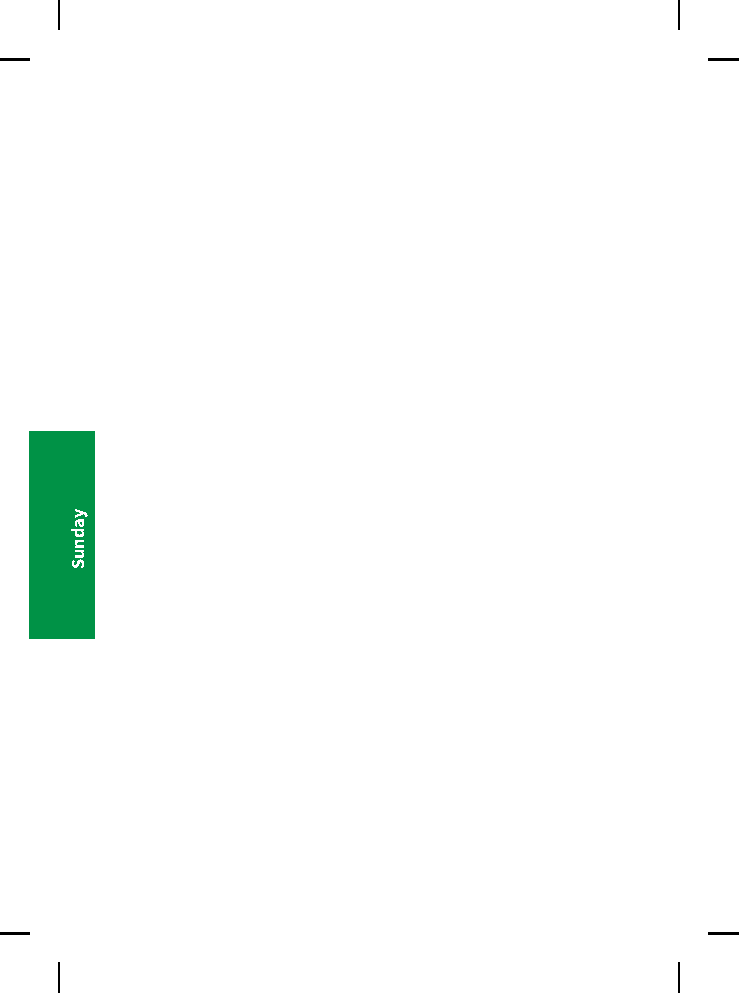
\includegraphics{wallpaper/sunday-even.pdf}%
}]{sundayeven}
\DeclareNewLayer[background, oddpage,  width=125mm,%
height=169mm, contents={%
  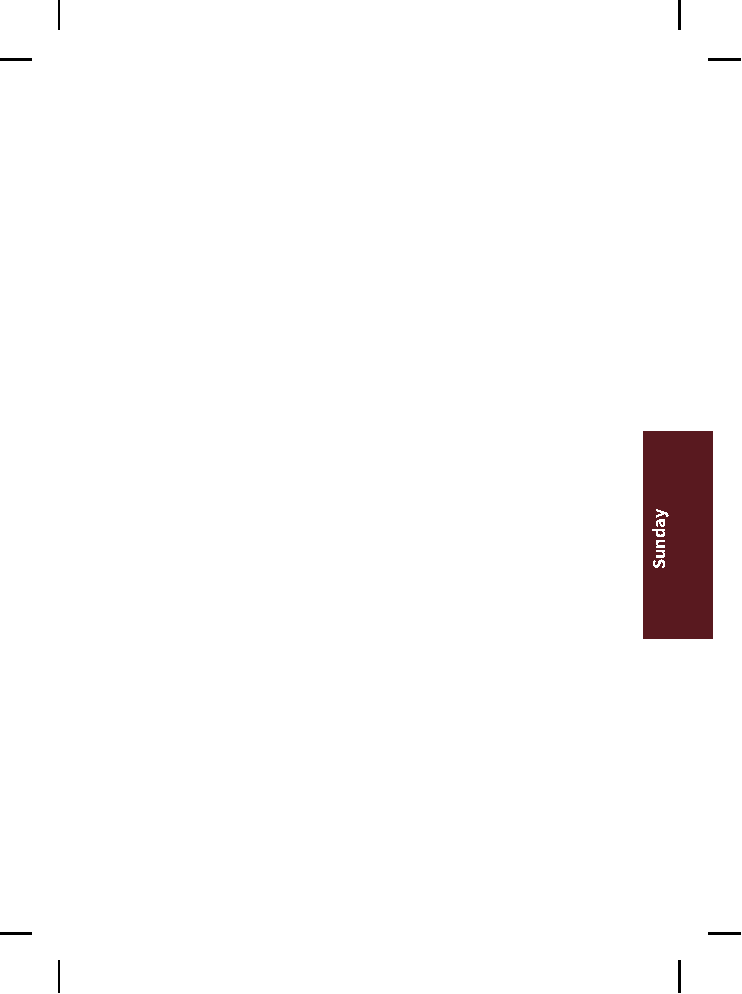
\includegraphics{wallpaper/sunday-odd-rotated.pdf}%
}]{sundayoddrotated}
\newpairofpagestyles[scrheadings]{sunday-table}{}
\AddLayersAtBeginOfPageStyle{sunday-table}{sundayeven}
\AddLayersAtBeginOfPageStyle{sunday-table}{sundayoddrotated}
\newpairofpagestyles[scrheadings]{sunday}{}
\AddLayersAtBeginOfPageStyle{sunday}{sundayeven}
\AddLayersAtBeginOfPageStyle{sunday}{sundayodd}

% define Monday page style
\DeclareNewLayer[background, oddpage,  width=125mm,%
height=169mm, contents={%
  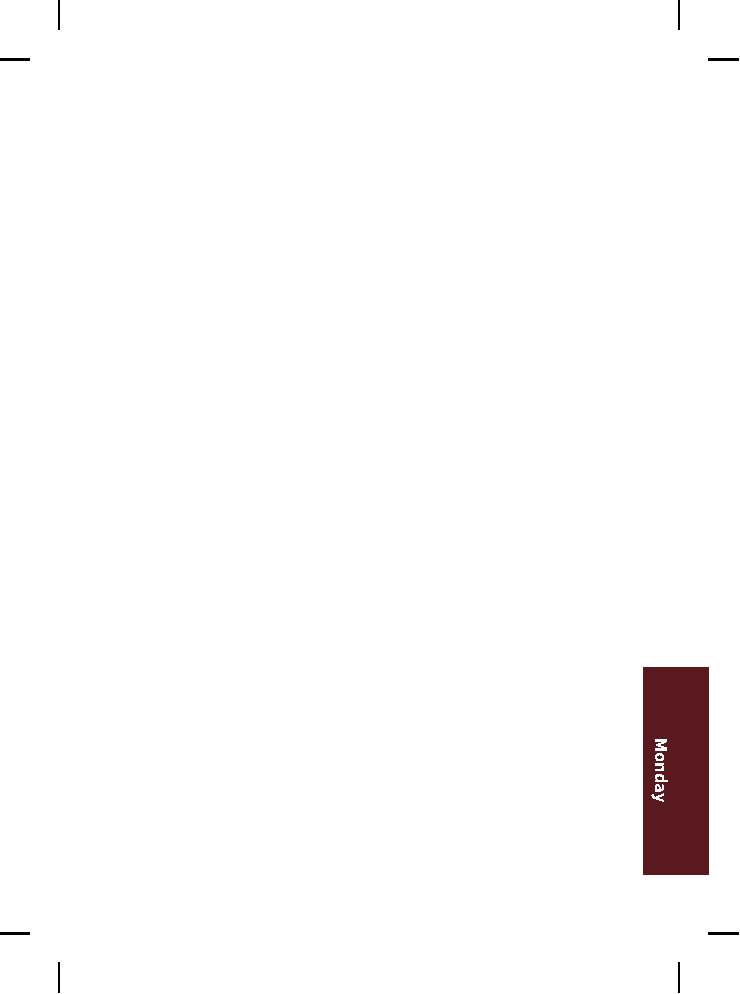
\includegraphics{wallpaper/monday-odd.pdf}%
}]{mondayodd}
\DeclareNewLayer[background, evenpage,  width=125mm,%
height=169mm, contents={%
  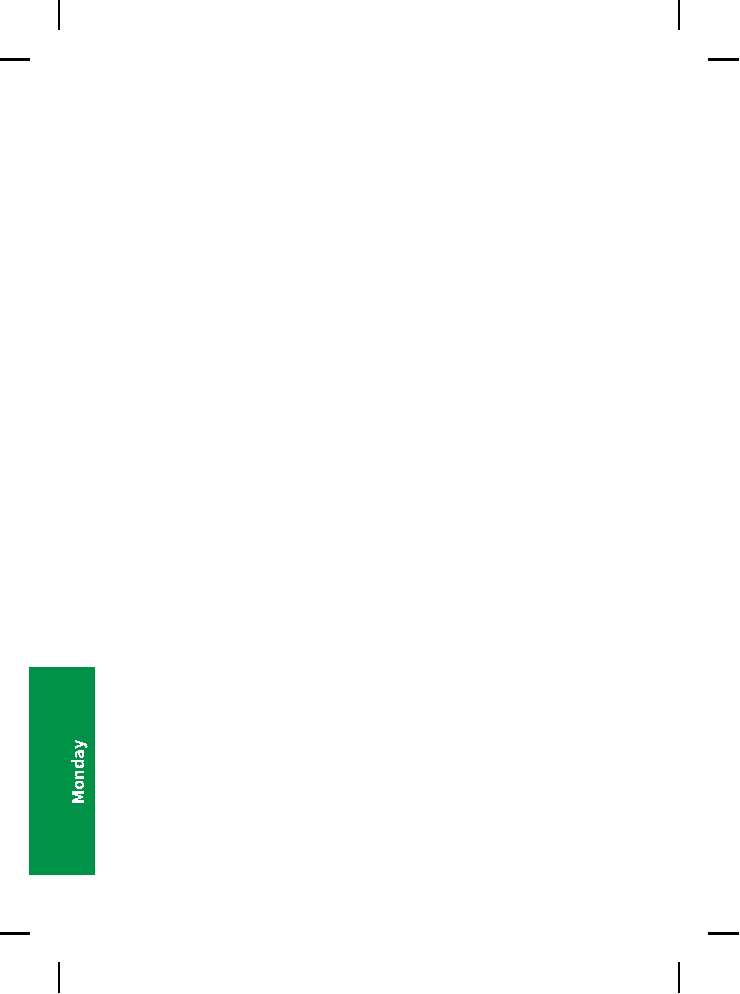
\includegraphics{wallpaper/monday-even.pdf}%
}]{mondayeven}
\DeclareNewLayer[background, oddpage,  width=125mm,%
height=169mm, contents={%
  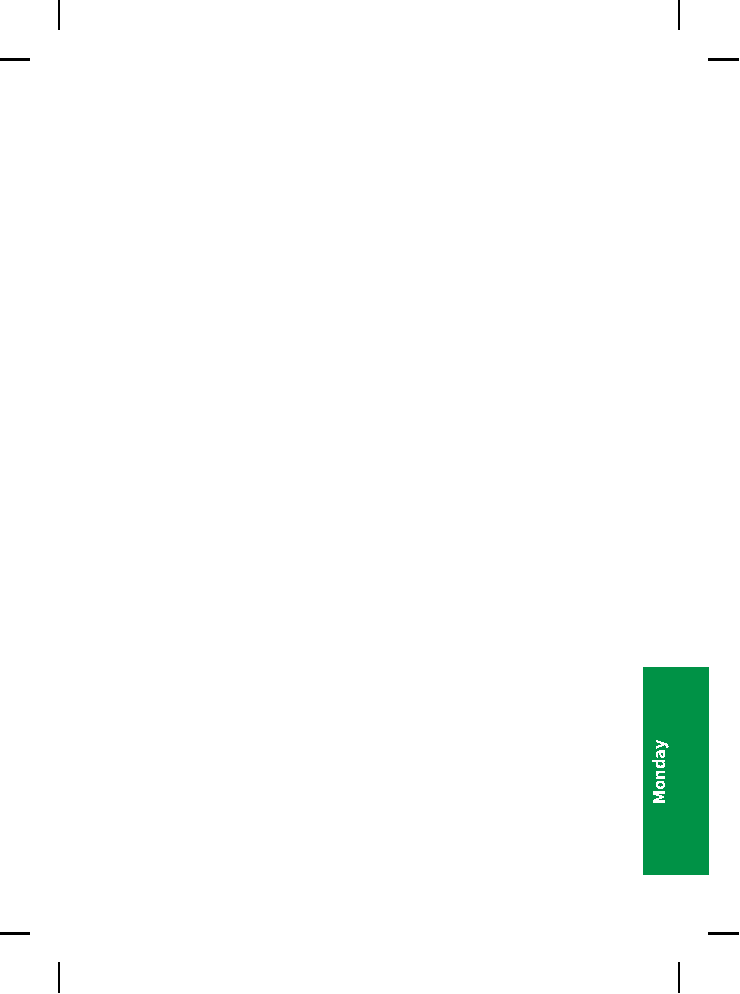
\includegraphics{wallpaper/monday-odd-rotated.pdf}%
}]{mondayoddrotated}
\newpairofpagestyles[scrheadings]{monday-table}{}
\AddLayersAtBeginOfPageStyle{monday-table}{mondayeven}
\AddLayersAtBeginOfPageStyle{monday-table}{mondayoddrotated}
\newpairofpagestyles[scrheadings]{monday}{}
\AddLayersAtBeginOfPageStyle{monday}{mondayeven}
\AddLayersAtBeginOfPageStyle{monday}{mondayodd}

% \setpagebackground selects the page style to be used depending on the current day. Each day has
% its own page style.
\newcommand{\setpagebackground}{ %
  \ifthenelse{\equal{\conferenceDay}{\saturday}}{%
    \pagestyle{saturday}
  }{}
  \ifthenelse{\equal{\conferenceDay}{\sunday}}{%
    \pagestyle{sunday}
  }{}
  \ifthenelse{\equal{\conferenceDay}{\monday}}{%
    \pagestyle{monday}
  }{}
}


% additional column type for tables
\newcolumntype{Y}[1]{>{\RaggedRight\arraybackslash}p{#1}}

%% length of the title boxes
\newlength{\titleboxwidth}
\setlength{\titleboxwidth}{\textwidth}
\advance\titleboxwidth by -6pt

% command to lay out the title boxes
\newcommand{\setAbstract}[6]{
  % 1. speaker
  % 2. title
  % 3. subtitle
  % 4. abstract (Text)
  % 5. colour
  % 6. room
  %\thispagestyle{scrheadings}
  \setPageBackground
  \setlength\tabcolsep{0pt}
  % \setlength{\fboxsep}{0pt}
  \noindent\fcolorbox{white}{#5}{%
    \parbox{\titleboxwidth}{%
      \noindent\begin{tabu}{X[5L]r}
        \isSpeakerEmpty{#1}{#2}{#6}
        \isSubtitleEmpty{#3}
      \end{tabu}%
    }%
  }%
  %
  \isAbstractEmpty{#4}%
  \vspace{0.5em}% space to the next talk even if there is no abstract
  \setlength\tabcolsep{6pt} % set column padding back to default value
}

% lay out the speaker if there is any
% We assume that there is only a subtitle if the talk has a speaker.
\makeatletter
  \newcommand{\isSpeakerEmpty}[3]{%
    % Arguments:
    % 1. speaker
    % 2. title
    % 3. room
    \@ifmtarg{#1}{%
      \par\noindent\large \sectfont #2% % titel
      &
      #3, \talkTime
      \tabularnewline
    }%
    {
      \emph{#1} % Sprecher
      &
      \talkTime
      \tabularnewline
      {%
        \par\noindent\large \sectfont #2%
      }% % titel
      &
      #3
      \tabularnewline
    }%
  }
\makeatother

% Lay out the subtitle
% has to be a separate function and has to be surrounded by \makeatletter for technical reasons
\makeatletter
  \newcommand{\isSubtitleEmpty}[1]{%
    \@ifnotmtarg{#1}{%
      \multicolumn{2}{Y{\linewidth}}{%
        \vspace{-0.6em}%
        \noindent%
        \bfseries
        \normalsize
        \sectfont #1%
      }
      \tabularnewline%
    }
  }
\makeatother

% Lay out the abstract if there is any
% has to be a separate function and has to be surrounded by \makeatletter for technical reasons
\makeatletter
\newcommand{\isAbstractEmpty}[1]{%
  \ifstrempty{#1}{%
    \vspace{1.5em}%
  }{%
    \vspace{0.5em}\newline%
    #1 \par% % abstract
    \vspace{1.5em}% space to the next talk even if there is an abstract
  }%
}
\makeatother

% define colours
\definecolor{GHS}{cmyk}{0.16 0 .05 0}
\definecolor{HSO}{cmyk}{0.02 0 0.12 0.11}
\definecolor{academic}{cmyk}{0 0.02 0.23 0}
\definecolor{HSW}{cmyk}{0.35 0 0.33 0.16}
\definecolor{KHS}{cmyk}{0 .24 0.29 .04}
\definecolor{Mathematikon C}{cmyk}{.16 0 0.35 0}
\definecolor{ochsenblutrot}{cmyk}{0 0.72 0.65 0.65}

% session at GHS
\newcommand{\abstractGHS}[4]%
{%
  \setAbstract{#1}{#2}{#3}{#4}{GHS}{GHS}
}

% abstract at HSO 
\newcommand{\abstractHSO}[4]%
{%
  \setAbstract{#1}{#2}{#3}{#4}{HSO}{HSO}
}

% abstract for academic talks
\newcommand{\abstractAcademic}[4]%
{%
  \setAbstract{#1}{#2}{#3}{#4}{academic}{HSW}
}

% abstract at HSW
\newcommand{\abstractHSW}[4]%
{%
  \setabstract{#1}{#2}{#3}{#4}{HSW}{HSW}
}

% abstract at KHS
\newcommand{\abstractKHS}[4]%
{%
  \setabstract{#1}{#2}{#3}{#4}{KHS}{KHS}
}

% abstract at Mathematikon C
\newcommand{\abstractMathematikonC}[4]%
{%
  \setabstract{#1}{#2}{#3}{#4}{Mathematikon C}{Mathematikon C}
}

% abstract at a different location
\newcommand{\abstractOther}[5]%
{%
  \setAbstract{#1}{#2}{#3}{#4}{commongray}{#5}
}

% infobox for workshops (they don't have an abstract in the booklet)
\newcommand{\workshopbox}[3]{%
  % 1. titel
  % 2. speaker
  % 3. Room
  \setlength\tabcolsep{0pt}
  \noindent\fcolorbox{white}{dezentrot}{%
    \parbox{\titleboxwidth}{%
      \noindent%
      \begin{tabu}{X[5L]r}
        \emph{#2} % Sprecher
        &
        \talkTime
        \tabularnewline
        {\noindent\large \bfseries #1}% % title
        &
        #3
        \tabularnewline
      \end{tabu}
    }
  }
  \setlength\tabcolsep{6pt} % set column padding back to default
}

% too long
\newcommand{\tooLong}{Dieser Text ist viel zu lang. Dieser Text ist viel zu lang. Dieser Text ist viel zu lang. Dieser Text ist viel zu lang. Dieser Text ist viel zu lang. Dieser Text ist viel zu lang. Dieser Text ist viel zu lang. Dieser Text ist viel zu lang. Dieser Text ist viel zu lang. Dieser Text ist viel zu lang. Dieser Text ist viel zu lang. Dieser Text ist viel zu lang. Dieser Text ist viel zu lang. Dieser Text ist viel zu lang. }

\newlength{\fboxwidth}

\def\workshopsSection{workshopsSection}
\def\abstractsSection{abstractsSection}

% boxes for text-only advertisement texts by our sponsors
\newcommand{\sponsorBox}[4]{%
  \setlength{\fboxwidth}{\textwidth}
  \advance\fboxwidth by -7.0pt
  \abstractSponsorbox{#1}{#2}{#3}{#4}{\workshopsSection}%
}

\newcommand{\sponsorBoxA}[4]{%
  \setlength{\fboxwidth}{\textwidth}
  \advance\fboxwidth by -10.0pt
  \abstractSponsorbox{#1}{#2}{#3}{#4}{\abstractsSection}%
}

%% store \parindent in separate variable because it is resetted to 0 in parboxes
\newlength{\saveparindent}
\setlength{\saveparindent}{\parindent}

%% box for advertisment by a sponsor
%% 1. logo
%% 2. width of the logo
%% 3. number of required lines of the logo (due to usage of wrapfigure)
%% 4. text
%% 5. Umfeld (\workshopsSection oder \abstractsSection}
\makeatletter
  \newcommand{\abstractSponsorbox}[5]{%
    \setlength{\fboxsep}{4.5pt}%
    \noindent%
    \ifthenelse{\equal{#5}{\workshopsSection}}{%
      \hspace{2.65pt}%
    }{%
      \hspace{-1pt}%
    }%
    \fcolorbox{gray}{white}{%
      \parbox{\fboxwidth}{
        \setlength{\parindent}{\saveparindent}%
        \@ifmtarg{#1}{}{%
          \begin{wrapfigure}[#3]{r}[0pt]{#2}
            \centering\vspace{-1\baselineskip}
            \includegraphics[width=#2]{#1}
          \end{wrapfigure}
        }
  
        \noindent #4
      }%
    }
    \setlength{\fboxsep}{3pt}
  }
  \setlength{\fboxsep}{3pt}
\makeatother

% definition of column types for the schedule tables
\newcolumntype{Z}[1]{>{\RaggedRight\arraybackslash}p{#1}}%
\newcolumntype{C}[1]{>{\Centering\arraybackslash}p{#1}}%

% common implementation of typesetting of a session in the tables
\newcommand{\talkInternal}[2]{%
  \textbf{#1}
  \ifthenelse{\equal{#2}{}}{}{%
    \newline\emph{#2}%
  }
}

% macro to typeset a talk in the schedule tables spanning over more than one row:
% usage: \longTalk{rowcount}{title}{speaker}
\newcommand{\longTalk}[3]{%
  &
  \multirow{#1}{\linewidth}{%
    \parbox{\linewidth}{
      %HACK Inserting a \vspace here is a dirty hack but it works.
      \vspace{0.45\baselineskip}
      \talkInternal{#2}{#3}%
    }
  }%
}%

% macro to typeset a talk in the schedule tables:
% usage: \talk{title}{speaker}
\newcommand{\talk}[2]{%
  &
  \talkInternal{#1}{#2}%
}%


% macro to typeset a talk in the schedule tables spanning over more than one column:
% usage: \multiColTalk{columns}{columnSpecs}{title}{speaker}
\newcommand{\multiColTalk}[4]{%
  &
  \multicolumn{#1}{#2}{\talkInternal{#3}{#4}}%
}%

\newcommand{\workshop}[3]%
{%
  \workshopbox{#1}{#2}{#3}
}%

\newcommand{\otherevent}[1]%
{%
  & \textbf{#1}
}%

\newcommand{\audimaxEvent}[2]%
{%
  &
  \multicolumn{3}{c}{
    \textbf{#1} (Audimax) \par \emph{#2}
  }
}%

\newcommand{\coffeespace}{\vspace{0.4em}}
\newcommand{\workshopspace}{\vspace{0.5em}\\}

% define colors
\definecolor{commongray}{gray}{.9}
\definecolor{tableRuleGray}{gray}{.4}
\definecolor{textGray}{gray}{.45}

% macro for table rules
\newcommand{\programCRule}[1]{%
  \arrayrulecolor{tableRuleGray}%
  \cdashline{#1}[0.2mm/2mm]%
}
\newcommand{\programHRule}[1]{%
  \arrayrulecolor{tableRuleGray}%
  \cdashline{2-#1}[0.2mm/2mm]%
}

% macro for empty session slots
\newcommand{\bookableSpace}{
  & \emph{\textcolor{textGray}{bookable space}}%
}

% diamond symbol for shortened titles
\newcommand{\diamondSymbol}{%
  \textsuperscript{%
    \diamond%
  }%
}

% macro for no-video icon
% Argument: height
\newcommand{\noVideo}[1]{%
  \includegraphics[height=#1]{no-video.pdf}%
}
